\documentclass[]{article}
\usepackage{lmodern}
\usepackage{amssymb,amsmath}
\usepackage{ifxetex,ifluatex}
\usepackage{fixltx2e} % provides \textsubscript
\ifnum 0\ifxetex 1\fi\ifluatex 1\fi=0 % if pdftex
  \usepackage[T1]{fontenc}
  \usepackage[utf8]{inputenc}
\else % if luatex or xelatex
  \ifxetex
    \usepackage{mathspec}
  \else
    \usepackage{fontspec}
  \fi
  \defaultfontfeatures{Ligatures=TeX,Scale=MatchLowercase}
\fi
% use upquote if available, for straight quotes in verbatim environments
\IfFileExists{upquote.sty}{\usepackage{upquote}}{}
% use microtype if available
\IfFileExists{microtype.sty}{%
\usepackage{microtype}
\UseMicrotypeSet[protrusion]{basicmath} % disable protrusion for tt fonts
}{}
\usepackage[margin=1in]{geometry}
\usepackage{hyperref}
\hypersetup{unicode=true,
            pdftitle={Interactive lecture module 8 and 9 - solutions},
            pdfauthor={Mette Langaas},
            pdfborder={0 0 0},
            breaklinks=true}
\urlstyle{same}  % don't use monospace font for urls
\usepackage{graphicx,grffile}
\makeatletter
\def\maxwidth{\ifdim\Gin@nat@width>\linewidth\linewidth\else\Gin@nat@width\fi}
\def\maxheight{\ifdim\Gin@nat@height>\textheight\textheight\else\Gin@nat@height\fi}
\makeatother
% Scale images if necessary, so that they will not overflow the page
% margins by default, and it is still possible to overwrite the defaults
% using explicit options in \includegraphics[width, height, ...]{}
\setkeys{Gin}{width=\maxwidth,height=\maxheight,keepaspectratio}
\IfFileExists{parskip.sty}{%
\usepackage{parskip}
}{% else
\setlength{\parindent}{0pt}
\setlength{\parskip}{6pt plus 2pt minus 1pt}
}
\setlength{\emergencystretch}{3em}  % prevent overfull lines
\providecommand{\tightlist}{%
  \setlength{\itemsep}{0pt}\setlength{\parskip}{0pt}}
\setcounter{secnumdepth}{0}
% Redefines (sub)paragraphs to behave more like sections
\ifx\paragraph\undefined\else
\let\oldparagraph\paragraph
\renewcommand{\paragraph}[1]{\oldparagraph{#1}\mbox{}}
\fi
\ifx\subparagraph\undefined\else
\let\oldsubparagraph\subparagraph
\renewcommand{\subparagraph}[1]{\oldsubparagraph{#1}\mbox{}}
\fi

%%% Use protect on footnotes to avoid problems with footnotes in titles
\let\rmarkdownfootnote\footnote%
\def\footnote{\protect\rmarkdownfootnote}

%%% Change title format to be more compact
\usepackage{titling}

% Create subtitle command for use in maketitle
\newcommand{\subtitle}[1]{
  \posttitle{
    \begin{center}\large#1\end{center}
    }
}

\setlength{\droptitle}{-2em}

  \title{Interactive lecture module 8 and 9 - solutions}
    \pretitle{\vspace{\droptitle}\centering\huge}
  \posttitle{\par}
  \subtitle{TMA4268 Statistical learning}
  \author{Mette Langaas}
    \preauthor{\centering\large\emph}
  \postauthor{\par}
      \predate{\centering\large\emph}
  \postdate{\par}
    \date{15 March, 2019}


\begin{document}
\maketitle

{
\setcounter{tocdepth}{2}
\tableofcontents
}
\section{8. Tree-based methods}\label{tree-based-methods}

\subsection{Problems for interactive
lecture}\label{problems-for-interactive-lecture}

\subsection{Problem 1: Regions and
tree}\label{problem-1-regions-and-tree}

We have a classification problem with covariates (predictors)
\texttt{Sepal.Width} and \texttt{Sepal.Length} and reponse
\texttt{Species} (three species)

The graph below gives a partition of the predictor space of variables
\texttt{Sepal.Width} and \texttt{Sepal.Length}, where the observations
are shown in different colors for the different species

\subsubsection{a) From regions to tree}\label{a-from-regions-to-tree}

Sketch the classification tree corresponding to the partition. Specify
variables that are split on and an approximate value of the split point

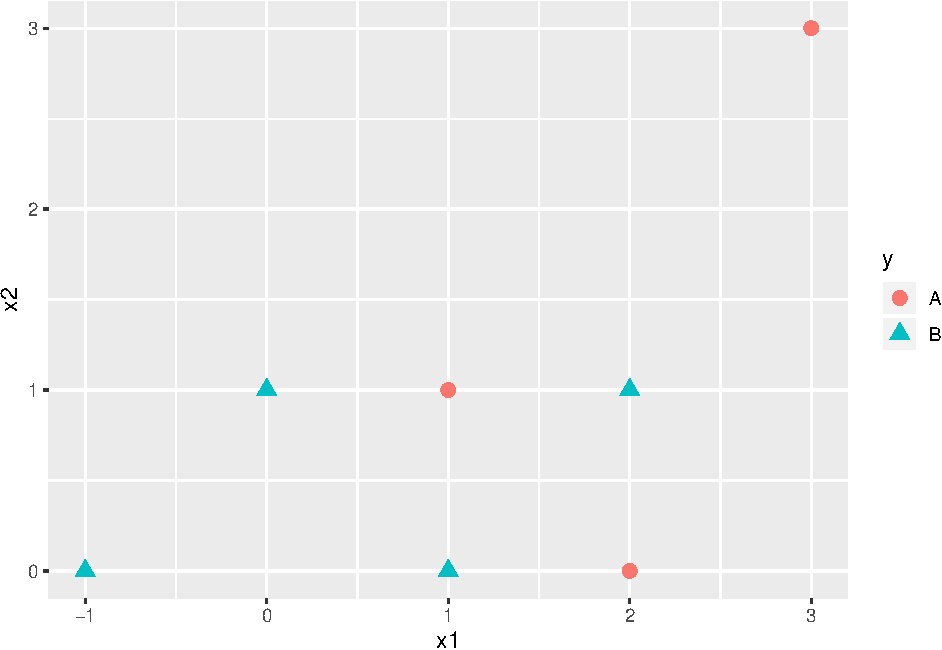
\includegraphics{89il-sol_files/figure-latex/unnamed-chunk-1-1.pdf}
\includegraphics{89il-sol_files/figure-latex/unnamed-chunk-1-2.pdf}

\subsubsection{b) From tree to regions}\label{b-from-tree-to-regions}

For the tree plot, draw the corresponding region plot.

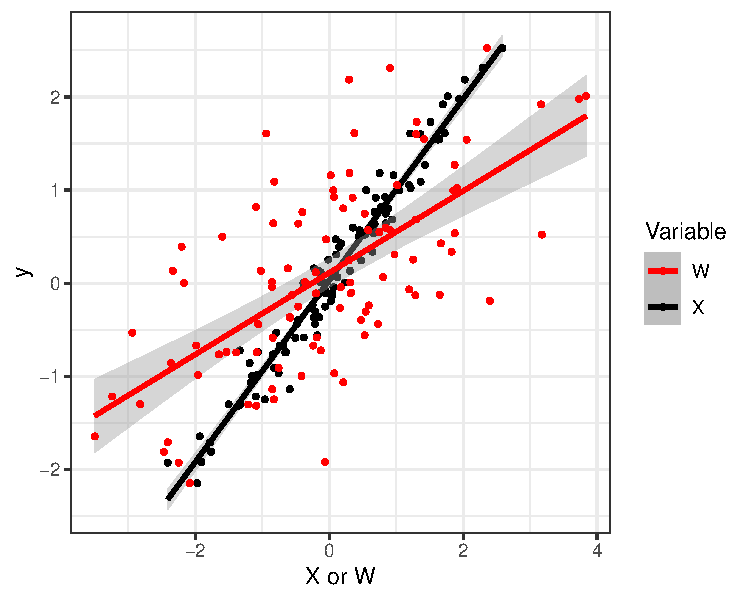
\includegraphics{89il-sol_files/figure-latex/unnamed-chunk-2-1.pdf}
\includegraphics{89il-sol_files/figure-latex/unnamed-chunk-2-2.pdf}

\subsection{Compulsory exercise 3 in 2018: Problem 1 on Classification
with
trees}\label{compulsory-exercise-3-in-2018-problem-1-on-classification-with-trees}

\url{https://www.math.ntnu.no/emner/TMA4268/2018v/CompEx/Compulsory3solutions.html}

\section{9. Support vector machines}\label{support-vector-machines}

\subsection{Compulsory exercise 3 in 2018: Problem
3:}\label{compulsory-exercise-3-in-2018-problem-3}

\url{https://www.math.ntnu.no/emner/TMA4268/2018v/CompEx/Compulsory3solutions.html}


\end{document}
